\begin{figure*}[hb]
  \centering

  \begin{subfigure}[t]{0.475\tw}\centering
    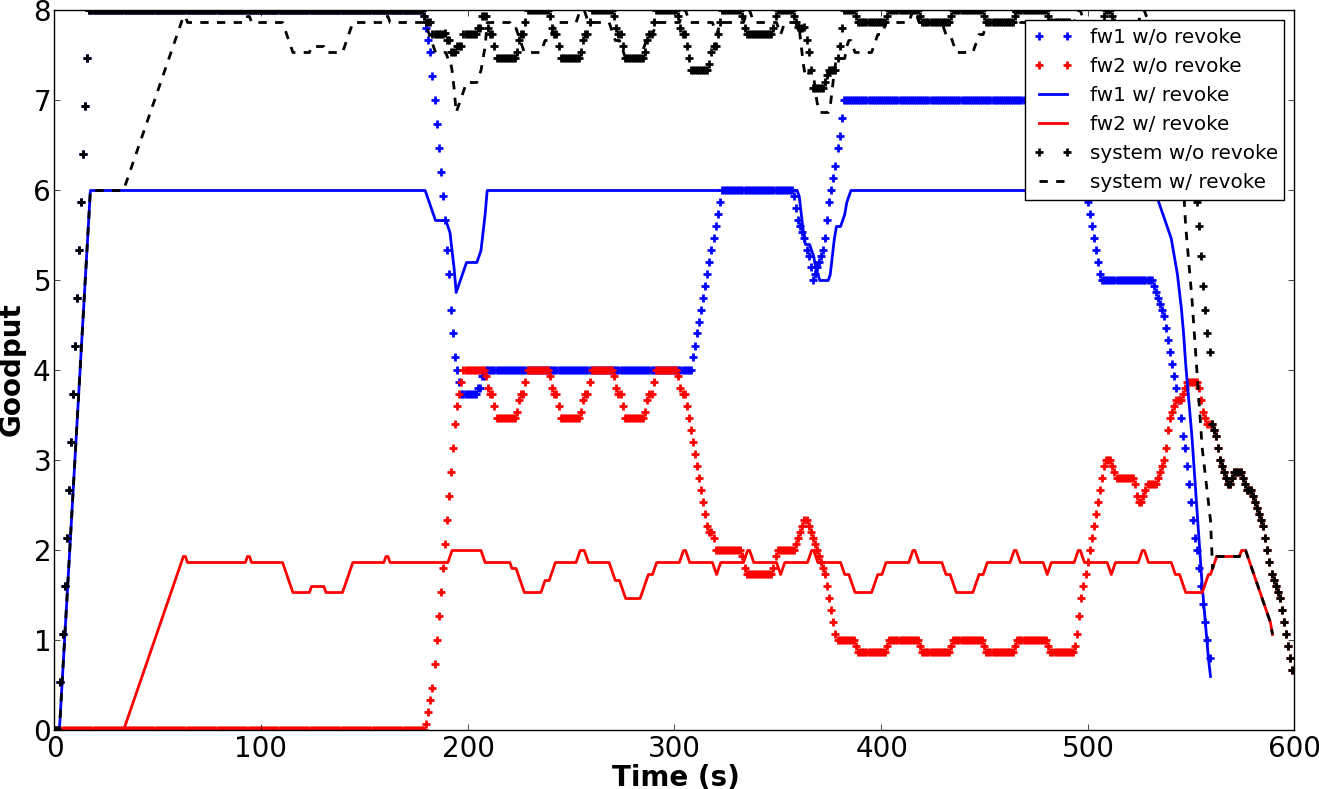
\includegraphics[width=\textwidth]{../results/30_goodput.png}
    \caption{Goodput Results for Scenario B}
    \label{fig:30-goodput}
  \end{subfigure}%
  \hfill
  \begin{subfigure}[t]{0.475\tw}\centering
    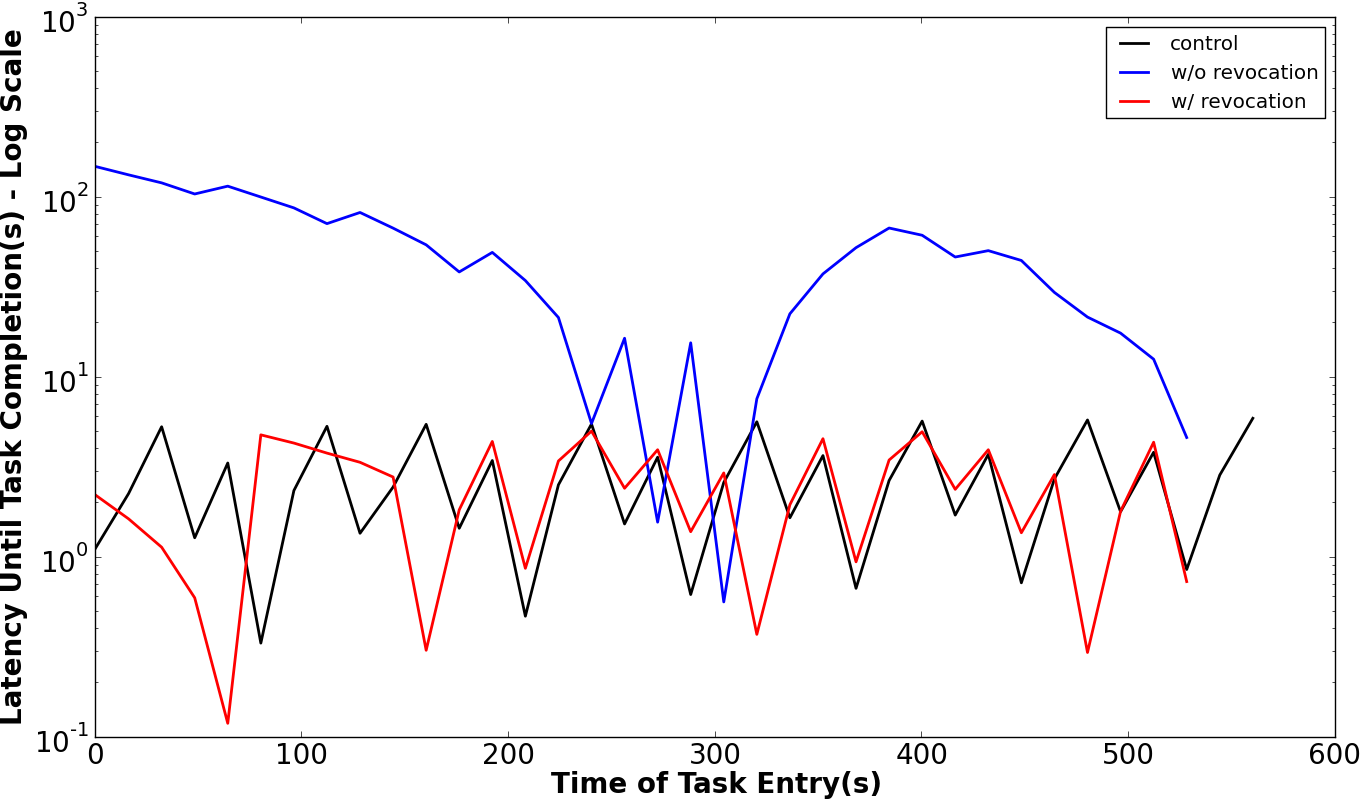
\includegraphics[width=\textwidth]{../results/30_fw_latency.png}
    \caption{Latency Results for Scenario B}
    \label{fig:30-latency}
  \end{subfigure}%

  \caption{\textbf{Goodput and Latency Results for Scenario B}
  In Figure~\ref{fig:30-goodput}, black lines correspond to the system's goodput, blue lines
  correspond to Framework 1's goodput, and red lines correspond to Framework 2's goodput. For the system
  goodput result, the $+$ lines correspond to the case without resource revocation and the dashed line
  corresponds to the cae with resource revocation. For the frameworks, the $+$ lines correspond to the
  case without resource revocation while the solid lines correspond to the case with resource
  revocation.
  Figure~\ref{fig:30-latency} plots Framework B's task latency when it is running in isolation
  (the black line), when it is running without resource revocation (the blue line), and when it is
  running with resource revocation (the red line).
  }
  \label{fig:30-goodput-latency}
\end{figure*}
